% lint-skip: 未完成ステータス（figure/table caption 未対応，人手チェック時に解消予定）
\documentclass[../../main.tex]{subfiles}
\begin{document}

\begin{flushright}
  \footnotesize\textit{【自動文字起こし・要確認】}
\end{flushright}

{\bf [解答]} $c = \cos t, s = \sin t$とする．題意の接線は $(\cos x)' = -\sin x$より，$y = -s(x-t) + c$だから，これと$x, y$軸との交点$A, B$として，$A(t + \dfrac{c}{s}, 0), B(0, c+st)$である．（$\because$ 接線は$y$軸平行でない）
\begin{figure}[H]
  \centering
  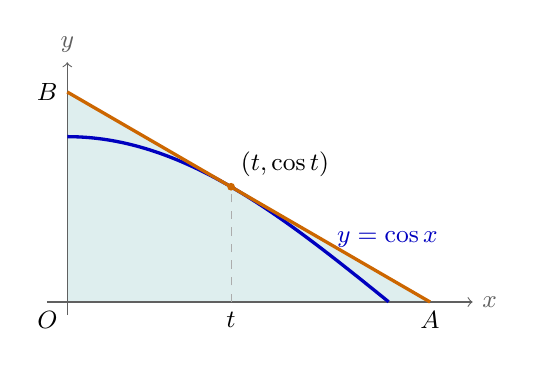
\begin{tikzpicture}[x=2.6cm,y=2.1cm,every node/.style={font=\small}]
    % t=0.8 の配置例．接線の x, y 切片は約1.77, 1.27．
    \coordinate (O) at (0,0);
    \coordinate (A) at (1.772,0);
    \coordinate (B) at (0,1.270);
    \coordinate (T) at (0.8,0.697);
    \fill[teal!13] (O)--(A)--(B)--cycle;
    \draw[->,gray!75!black] (-0.1,0)--(1.98,0) node[right] {$x$};
    \draw[->,gray!75!black] (0,-0.08)--(0,1.45) node[above] {$y$};
    \draw[blue!75!black,very thick,domain=0:1.57,samples=80]
    plot (\x,{cos(\x r)});
    \draw[orange!80!black,very thick] (B)--(A);
    \draw[gray!65,dashed] (0.8,0)--(T);
    \fill[orange!80!black] (T) circle (1.4pt);
    \node[below left] at (O) {$O$};
    \node[below] at (A) {$A$};
    \node[left] at (B) {$B$};
    \node[below] at (0.8,0) {$t$};
    \node[above right] at (T) {$(t,\cos t)$};
    \node[blue!75!black,above right] at (1.27,0.27) {$y=\cos x$};
  \end{tikzpicture}
  \caption{$y=\cos x$の$x=t$における接線と三角形$OAB$}
\end{figure}

\paragraph{(1)}

$S(t) = (\triangle OAB\text{の面積}) = \dfrac{1}{2}\left(t + \dfrac{c}{s}\right)(c+st) = \dfrac{1}{2}\left(t + \dfrac{\cos t}{\sin t}\right)(\cos t + \sin t \cdot t)$
\paragraph{(2)}

$2S(t) = c\left(t+\dfrac{c}{s}\right)$であり，区間内では$t^2$は単調増加，$\dfrac{1}{s^2}$は単調減少だから，$c > 0$とあわせて，$S'(t)$は単調増加である．これと$S'(\dfrac{\pi}{4}) = \dfrac{\sqrt{2}}{4}(\dfrac{\pi}{4}-1) < 0$ ($\because \pi=3.14\dots$)，$S'(1) = \cos 1 (2 - \dfrac{1}{\sin^2 1}) > \cos 1 (2-2) = 0$ ($\because \dfrac{\pi}{4} < 1 < \dfrac{\pi}{2}$から，$\sin 1 > \sin\dfrac{\pi}{4}, \cos 1 > 0$)，及び$S'(t)$が連続であることから，中間値の定理より，$S'(t_0) = 0$（$\dfrac{\pi}{4} < t_0 < 1$）なる$t_0$が存在し，下表をうる．
\begin{center}
  \begin{table}[htb]
    \centering
    \begin{tabular}{|c|c|c|c|c|c|}
      \hline
      $t$ & $0$ & $\cdots$ & $t_0$ & $\cdots$ & $\pi/2$ \\ \hline
      $S'$ & & $-$ & $0$ & $+$ & \\ \hline
      $S$ & & $\searrow$ & & $\nearrow$ & \\ \hline
    \end{tabular}
  \end{table}
\end{center}
したがって，$S(t)$は$t=t_0$でminをとる．以上から示された．

\paragraph{(3)}

$S'(t_0) = 0$及び$\cos t_0 \neq 0$から
$$
1 + {t_0}^2 = \dfrac{1}{\sin^2 t_0} = 1 + \dfrac{1}{\tan^2 t_0} \cdots \text{\textcircled{1}}
$$
である．(1)から
$$
S(t) = ct + \dfrac{1}{2}\left(st^2 + \dfrac{c^2}{s}\right)
$$
だから，$c_0 = \cos t_0, s_0 = \sin t_0$として，
$$
S(t_0) = c_0 t_0 + \dfrac{1}{2}\left( s_0 {t_0}^2 - 1 + \dfrac{1}{s_0} \right)
$$
$$
= c_0 t_0 + \left( \dfrac{1}{s_0} - s_0 \right) \quad (\because \text{\textcircled{1}}) \cdots \text{\textcircled{2}}
$$
となる．ここで，
$$
\dfrac{1}{s_0} - s_0 = \dfrac{{c_0}^2}{s_0} = c_0 \cdot \dfrac{c_0}{s_0} = c_0 \cdot \dfrac{1}{\tan t_0} = c_0 \cdot t_0 \quad (\because \text{\textcircled{1}}, t_0, \tan t_0 > 0)
$$
だから\textcircled{2}に代入して，
$$
S(t_0) = 2 \cos t_0 \cdot t_0
$$
となる．ここで，$f(t) = 2 c \cdot t$とおくと，$f'(t) = 2(c - st) = 2c(1 - t \cdot \tan t)$から下表をうる．
\begin{center}
  \begin{table}[htb]
    \centering
    \begin{tabular}{|c|c|c|c|c|c|c|c|c|c|}
      \hline
      $t$ & $0$ & $\cdots$ & $\pi/4$ & $\cdots$ & $t_0$ & $\cdots$ & $1$ & $\cdots$ & $\pi/2$ \\ \hline
      $f'$ & $+$ & $+$ & $+$ & $+$ & $0$ & $-$ & $-$ & $-$ & \\ \hline
      $f$ & & $\nearrow$ & $f(\pi/4)$ & $\nearrow$ & & $\searrow$ & & $\searrow$ & \\ \hline
    \end{tabular}
  \end{table}
\end{center}
(\textcircled{1}から，$t_0 = \dfrac{1}{\tan t_0}$であり，又，$1 - t \tan t$は区間内で単調増加)
したがって，$f(\dfrac{\pi}{4}) < f(t_0) \Leftrightarrow \dfrac{\sqrt{2}}{4}\pi < S(t_0)$である．

\end{document}
